\documentclass[english,notitlepage]{revtex4-1}  % defines the basic parameters of the document
%For preview: skriv i terminal: latexmk -pdf -pvc filnavn



% if you want a single-column, remove reprint

% allows special characters (including æøå)
\usepackage[utf8]{inputenc}
%\usepackage[english]{babel}

%% note that you may need to download some of these packages manually, it depends on your setup.
%% I recommend downloading TeXMaker, because it includes a large library of the most common packages.

\usepackage{physics,amssymb}  % mathematical symbols (physics imports amsmath)
\include{amsmath}
\usepackage{graphicx}         % include graphics such as plots
\usepackage{xcolor}           % set colors
\usepackage{hyperref}         % automagic cross-referencing (this is GODLIKE)
\usepackage{listings}         % display code
\usepackage{subfigure}        % imports a lot of cool and useful figure commands
\usepackage{float}
%\usepackage[section]{placeins}
\usepackage{algorithm}
\usepackage[noend]{algpseudocode}
\usepackage{subfigure}
\usepackage{tikz}
\usetikzlibrary{quantikz}
% defines the color of hyperref objects
% Blending two colors:  blue!80!black  =  80% blue and 20% black
\hypersetup{ % this is just my personal choice, feel free to change things
	colorlinks,
	linkcolor={red!50!black},
	citecolor={blue!50!black},
	urlcolor={blue!80!black}}

%% Defines the style of the programming listing
%% This is actually my personal template, go ahead and change stuff if you want



%% USEFUL LINKS:
%%
%%   UiO LaTeX guides:        https://www.mn.uio.no/ifi/tjenester/it/hjelp/latex/
%%   mathematics:             https://en.wikibooks.org/wiki/LaTeX/Mathematics

%%   PHYSICS !                https://mirror.hmc.edu/ctan/macros/latex/contrib/physics/physics.pdf

%%   the basics of Tikz:       https://en.wikibooks.org/wiki/LaTeX/PGF/Tikz
%%   all the colors!:          https://en.wikibooks.org/wiki/LaTeX/Colors
%%   how to draw tables:       https://en.wikibooks.org/wiki/LaTeX/Tables
%%   code listing styles:      https://en.wikibooks.org/wiki/LaTeX/Source_Code_Listings
%%   \includegraphics          https://en.wikibooks.org/wiki/LaTeX/Importing_Graphics
%%   learn more about figures  https://en.wikibooks.org/wiki/LaTeX/Floats,_Figures_and_Captions
%%   automagic bibliography:   https://en.wikibooks.org/wiki/LaTeX/Bibliography_Management  (this one is kinda difficult the first time)
%%   REVTeX Guide:             http://www.physics.csbsju.edu/370/papers/Journal_Style_Manuals/auguide4-1.pdf
%%
%%   (this document is of class "revtex4-1", the REVTeX Guide explains how the class works)


%% CREATING THE .pdf FILE USING LINUX IN THE TERMINAL
%%
%% [terminal]$ pdflatex template.tex
%%
%% Run the command twice, always.
%% If you want to use \footnote, you need to run these commands (IN THIS SPECIFIC ORDER)
%%
%% [terminal]$ pdflatex template.tex
%% [terminal]$ bibtex template
%% [terminal]$ pdflatex template.tex
%% [terminal]$ pdflatex template.tex
%%
%% Don't ask me why, I don't know.

\begin{document}

\title{Title of the document}      % self-explanatory
\author{Your name(s) here}          % self-explanatory
\date{\today}                             % self-explanatory
\noaffiliation                            % ignore this, but keep it.


\maketitle 
	
\textit{List a link to your github link here!}
	
\section*{Problem 1}

\subsection*{Problem a}
Write a solution for problem 1a here.

\subsection*{Problem b}
write a solution for problem 1b here.

\section*{Problem 2}
Here's an equation with numbering
\begin{equation}
	\vb{F} = \dv{\vb{p}}{t},
\end{equation}
and one without numbering:
$$
\oint_C \vb{F}\cdot \dd \vb{r} = 0.
$$

Here's a figure which we refer to as figure \ref{fig:ref}.

\begin{figure}[h!]
	\centering %Centers the figure
	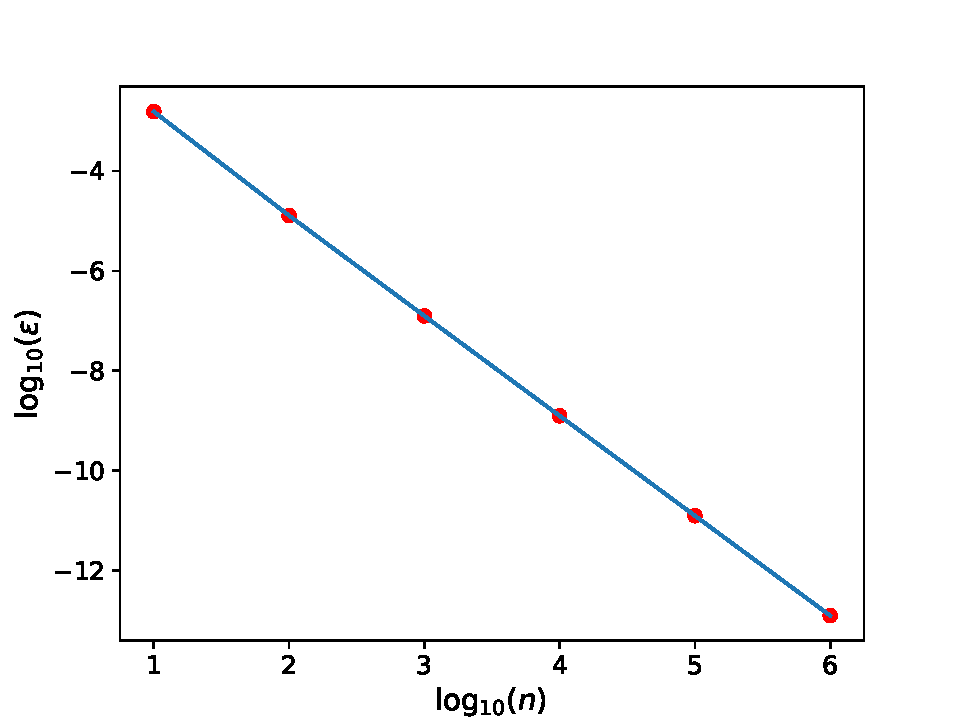
\includegraphics[scale=0.55]{imgs/rel_err.pdf} %Imports the figure.
	\caption{Write a descriptive caption here, explain its content. Note the size of the text on the axis and the ticks.}
	\label{fig:ref}
\end{figure}

Next up is a table. We refer to it by table \ref{tab:ref}

\begin{table}[h!]
	\centering
	\begin{tabular}{c@{\hspace{1cm}} c}
		\hline
		Number of points & Output \\
		\hline
		10 &  0.3086  \\
		
		100 &  0.2550\\
		\hline
	\end{tabular}\caption{Write a descriptive caption here, explaining the content of your table.}\label{tab:ref}
\end{table}

Finally, we can list algorithms by using 

\begin{algorithm}[H]
	\caption{Some algorithm}\label{algo:midpoint_rule}
	\begin{algorithmic}
		\State Some maths, e.g $f(x) = x^2$.  \Comment{Here's a comment}
		\For{$i = 0, 1, ..., n-1$}
		\State Do something here 
		\EndFor
		\While{Some condition}
		\State Do something more here 
		\EndWhile
		\State Maybe even some more math here, e.g $\int_0^1 f(x) \dd x$
	\end{algorithmic}
\end{algorithm}
	
	
\end{document}

